
\begin{figure*}
\centering
\begin{subfigure}{.485\textwidth}
  \centering
  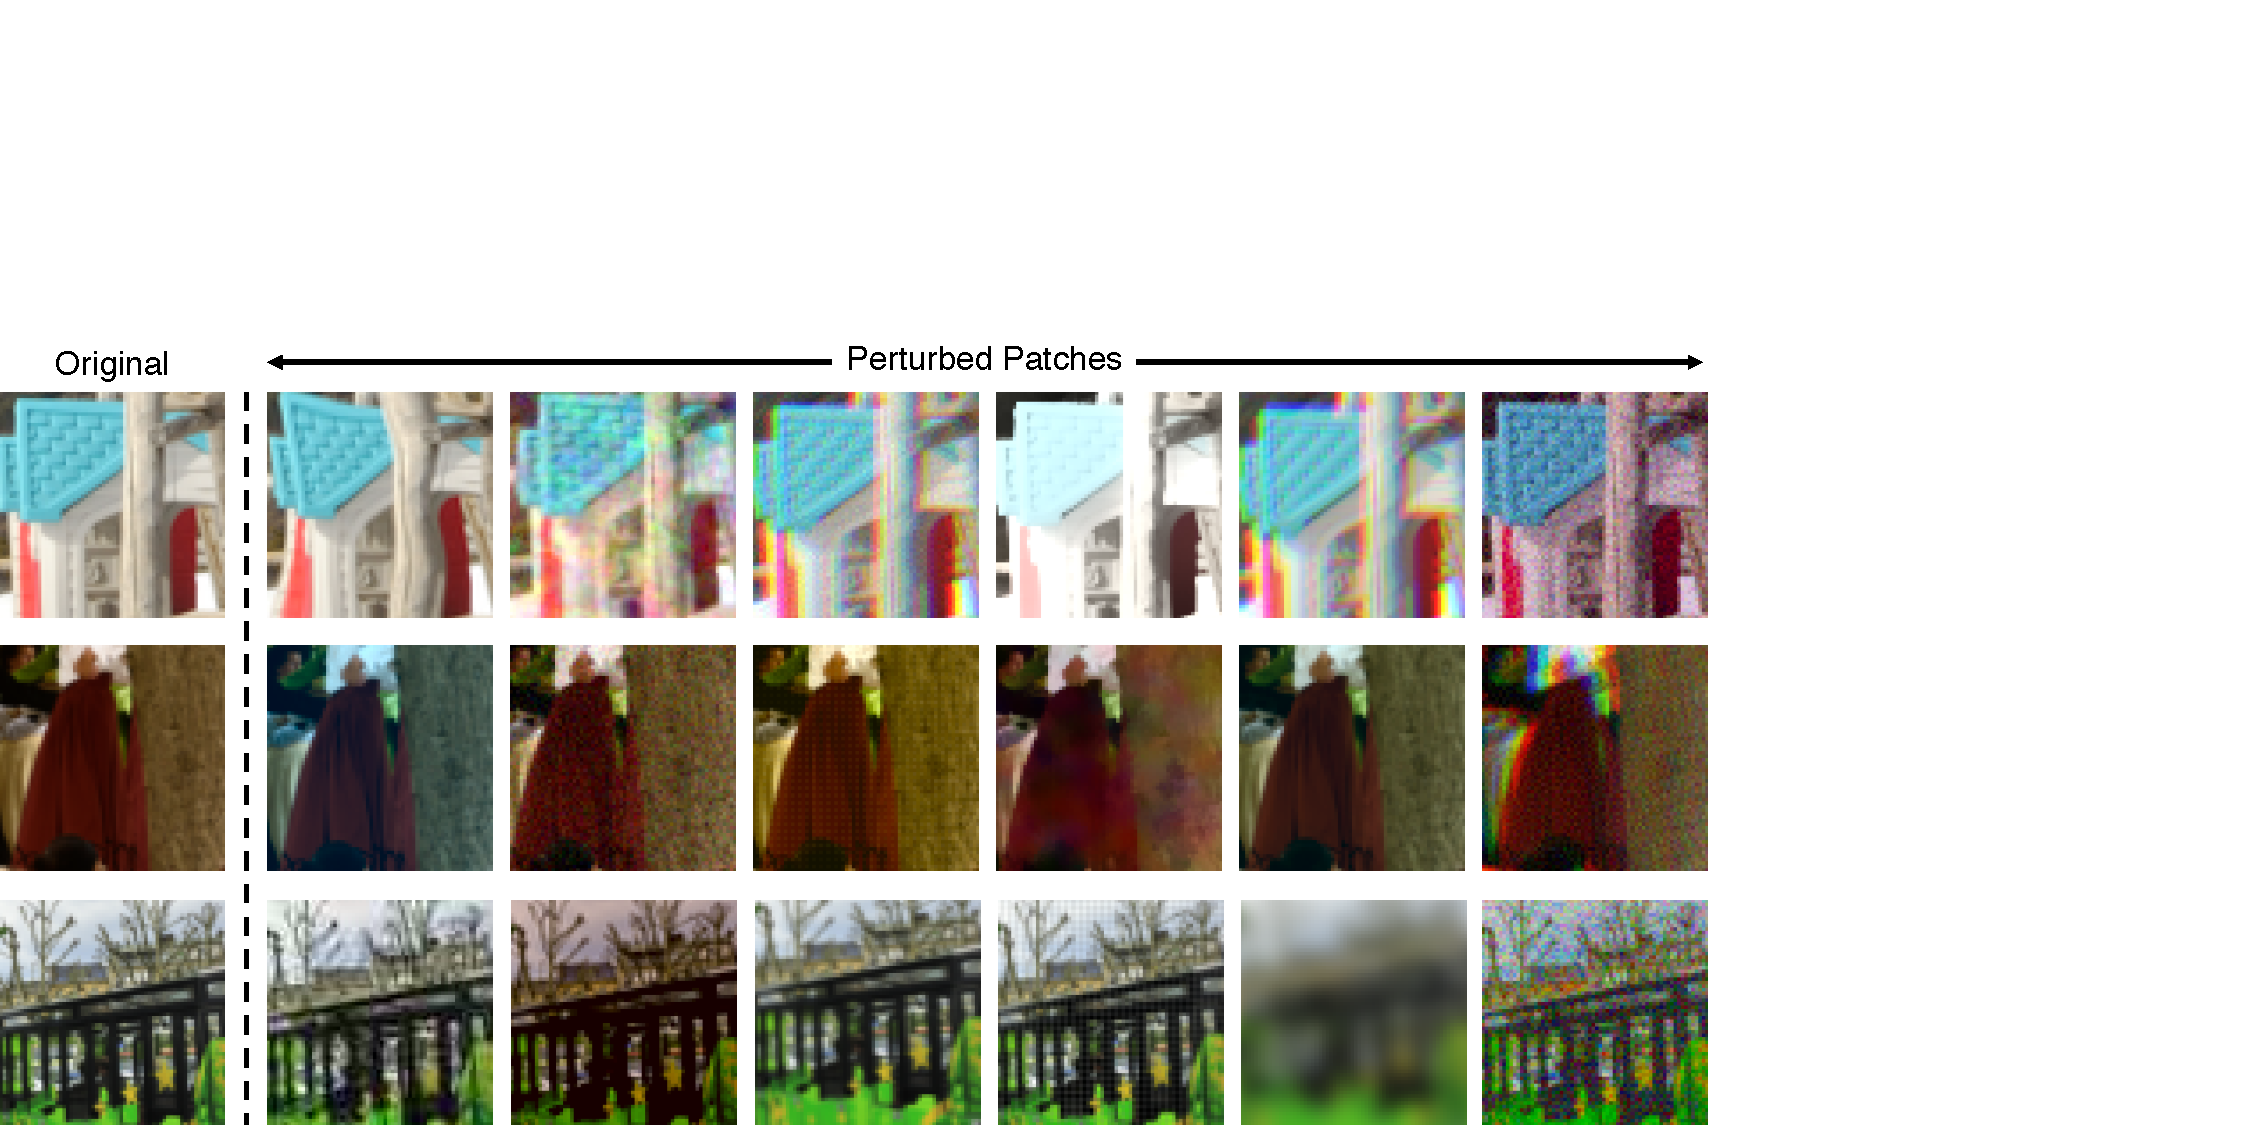
\includegraphics[width=1.\linewidth]{imgs/pert_lowlevel.pdf}
  \caption{\textbf{Traditional}}
  \label{fig:pert_low}
\end{subfigure}
\hspace{8px}
\begin{subfigure}{.485\textwidth}
  \centering
  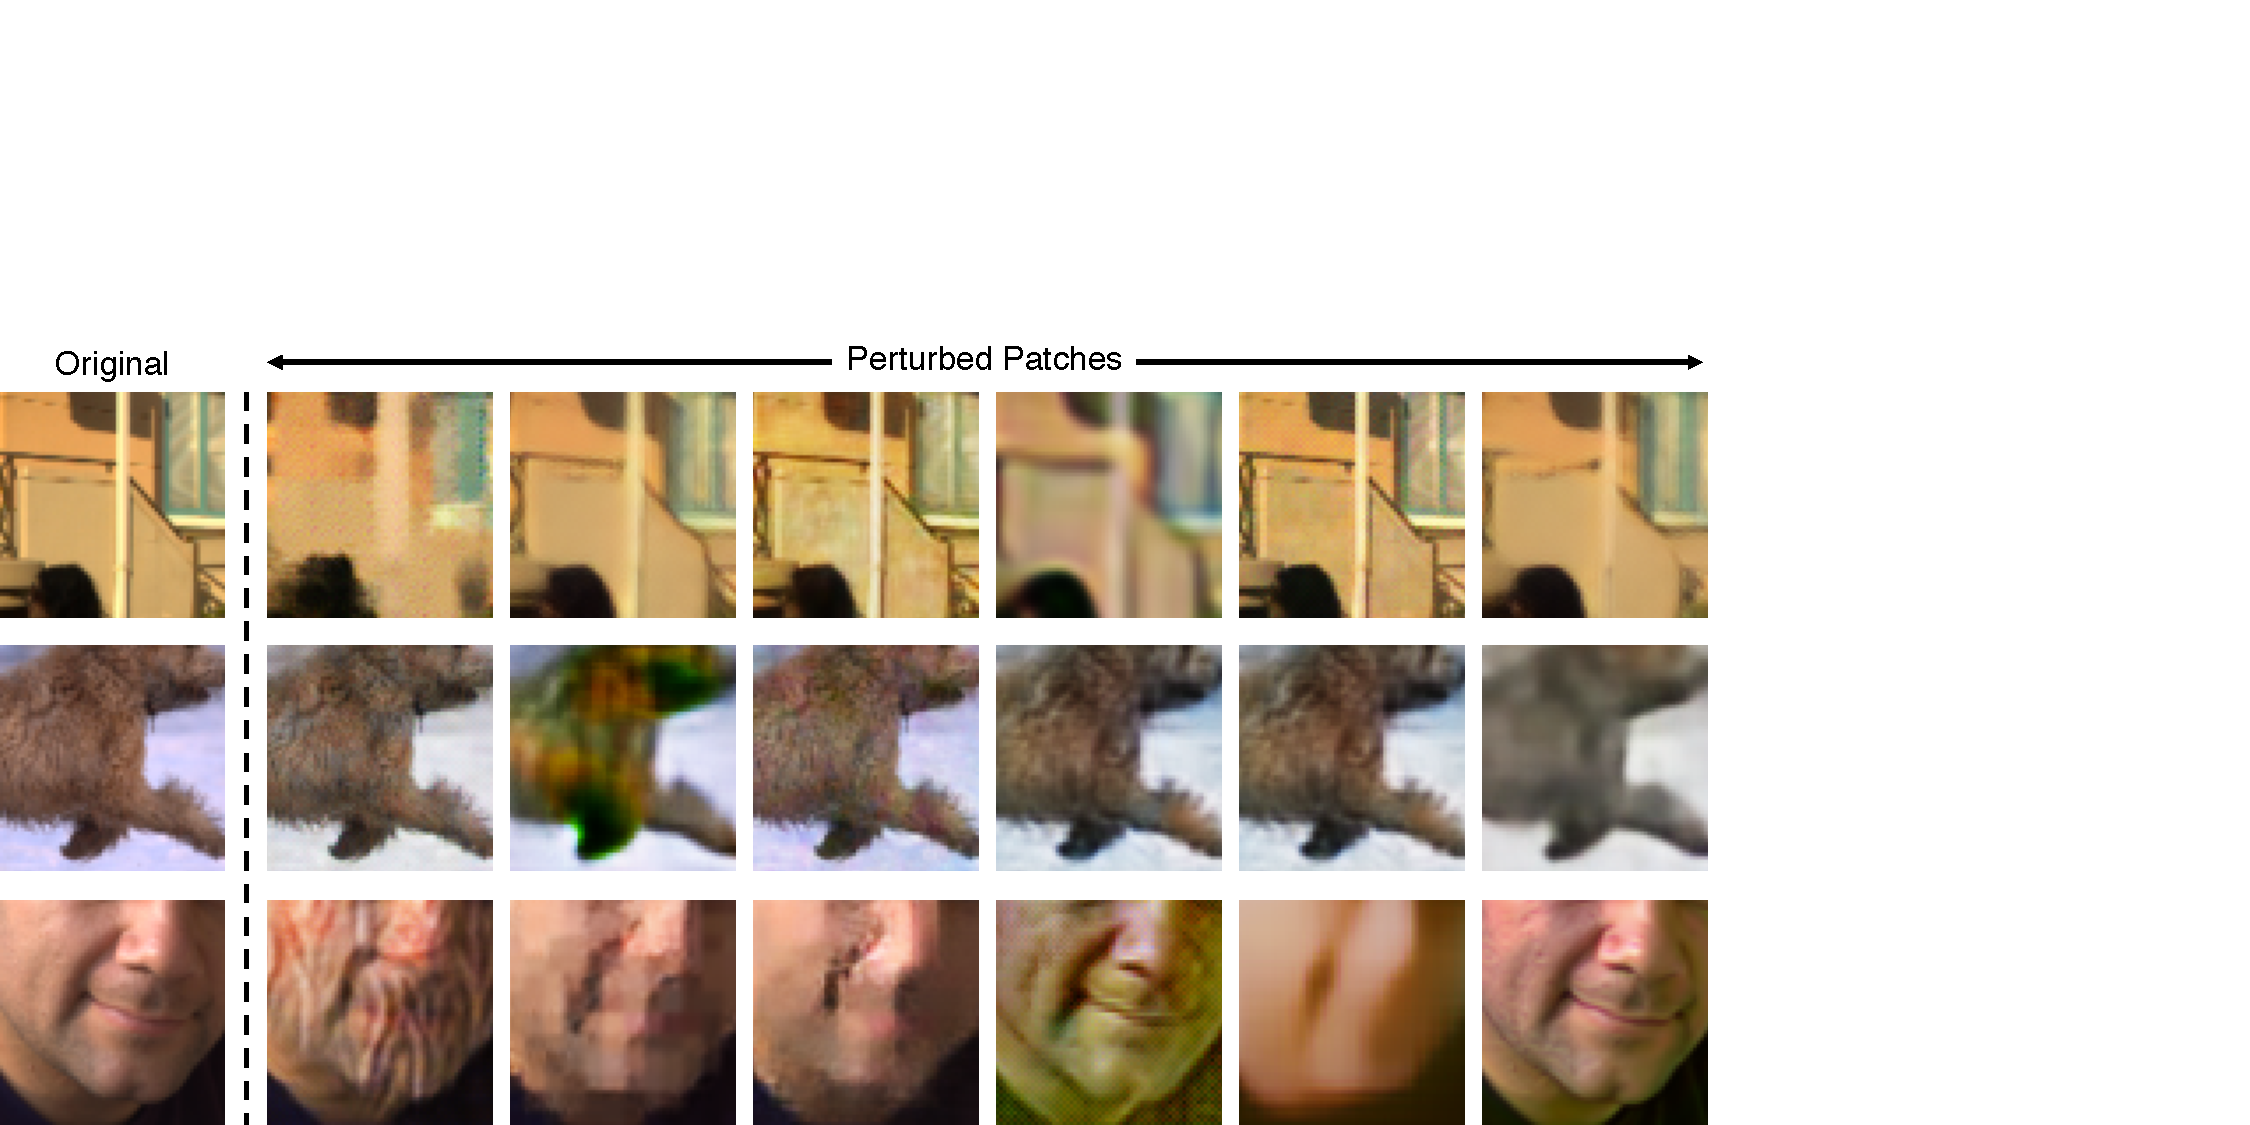
\includegraphics[width=1.\linewidth]{imgs/pert_highlevel.pdf}
  \caption{\textbf{CNN-based}}
  \label{fig:pert_high}
\end{subfigure}
\vspace{-2mm}
\caption{\textbf{Example distortions.} We show example distortions using our (a) traditional and (b) CNN-based methods.}
\vspace{-4mm}
\label{fig:pert}
\end{figure*}

\section{Motivation}

The ability to compare data items is perhaps the most fundamental operation underlying all of computing.  In many areas of computer science it does not pose much difficulty: one can use Hamming distance to compare binary patterns, edit distance to compare text files, Euclidean distance to compare vectors, etc.  The unique challenge of computer vision is that even this seemingly simple task of comparing visual patterns remains a wide-open problem.  Not only are visual patterns very high-dimensional and highly correlated, but, the very notion of visual similarity is often subjective, aiming to mimic human visual perception.  For instance, in image compression, the goal is for the compressed image to be indistinguishable from the original by a human observer, irrespective of the fact that their pixel representations might be very different. 

Classic per-pixel measures, such as $\ell_2$ Euclidean distance, commonly used for regression problems, or the related Peak Signal-to-Noise Ratio (PSNR), are insufficient for assessing structured outputs such as images, as they assume pixel-wise independence. A well-known example is that blurring causes large perceptual but small $\ell_2$ change.

What we would really like is a ``perceptual distance," which measures how similar are two images in a way that coincides with human judgment. This problem has been a longstanding goal,
%in the community
and there have been numerous perceptually motivated distance metrics proposed, such as SSIM~\cite{wang2004image}, MSSIM~\cite{wang2003multiscale}, FSIM~\cite{zhang2011fsim}, and HDR-VDP~\cite{mantiuk2011hdr}.

However, constructing a perceptual metric is challenging, because human judgments of similarity (1) depend on high-order image structure \cite{wang2004image}, (2) are context-dependent \cite{Goodman1972,medin1993respects,markman2005nonintentional}, and (3) may not actually constitute a distance metric \cite{tversky1977features}.
The crux of (2) is that there are many different ``senses of similarity" that we can simultaneously hold in mind: is a red circle more similar to a red square or to a blue circle? Directly fitting a function to human judgments may be intractable due the the context-dependent and pairwise nature of the judgments (which compare the similarity between \textit{two} images). Indeed, we show in this paper a negative result where this approach fails to generalize, even when trained on a large-scale dataset containing many distortion types.

Instead, might there be a way to learn a notion of perceptual similarity without directly training for it? The computer vision community has discovered that internal activations of deep convolutional networks, though trained on a high-level image classification task, are often surprisingly useful as a representational space for a much wider variety of tasks. For example, features from the VGG architecture~\cite{simonyan2014very} have been used on tasks such as neural style transfer~\cite{gatys2016image}, image superresolution~\cite{johnson2016perceptual}, and conditional image synthesis~\cite{dosovitskiy2016generating,chen2017photographic}. 
These methods measure distance in VGG feature space as a ``perceptual loss" for image regression problems~\cite{johnson2016perceptual,dosovitskiy2016generating}.

But how well do these ``perceptual losses'' actually correspond to human visual perception? How do they compare to traditional perceptual image evaluation metrics? Does the network architecture matter? Does it have to be trained on the ImageNet classification task, or would other tasks work just as well?  Do the networks need to be trained at all?

\subfile{tables/dataset_comparison}

In this paper, we evaluate these questions on a new large-scale database of human judgments, and arrive at several surprising conclusions. We find that internal activations of networks trained for high-level classification tasks, even across network architectures~\cite{iandola2016squeezenet,krizhevsky2012imagenet,simonyan2014very} and no further calibration, do indeed correspond to human perceptual judgments. In fact, they correspond far better than the commonly used metrics like SSIM and FSIM~\cite{wang2004image, zhang2011fsim}, which were not designed to handle situations where spatial ambiguities are a factor~\cite{sampat2009complex}. Furthermore, the best performing self-supervised networks, including BiGANs~\cite{donahue2016adversarial}, cross-channel prediction~\cite{zhang2017split}, and puzzle solving~\cite{noroozi2016unsupervised} perform just as well at this task, even without the benefit of human-labeled training data. Even a simple unsupervised network initialization with stacked k-means~\cite{krahenbuhl2015data} beats the classic metrics by a large margin! 
This illustrates an \textit{emergent property} shared across networks, even across architectures and training signals. Importantly, however, having \textit{some} training signal appears crucial -- a randomly initialized network achieves much lower performance.

Our study is based on a newly collected perceptual similarity dataset, using a large set of distortions and real algorithm outputs. It contains both traditional distortions, such as contrast and saturation adjustments, noise patterns, filtering, and spatial warping operations, and CNN-based algorithm outputs, such as autoencoding, denoising, and colorization, produced by a variety of architectures and losses. Our dataset is richer and more varied than previous datasets of this kind~\cite{ponomarenko2015image}. We also collect judgments on outputs from real algorithms for the tasks of superresolution, frame interpolation, and image deblurring, which is especially important as these are the real-world use cases for a perceptual metric.
We show that our data can be used to ``calibrate" existing networks, by learning a simple linear scaling of layer activations, to better match low-level human judgments.

Our results are consistent with the hypothesis that perceptual similarity is not a special function all of its own, but rather a {\em consequence} of visual representations tuned to be predictive about important structure in the world. Representations that are effective at semantic prediction tasks are also representations in which Euclidean distance is highly predictive of perceptual similarity judgments.

Our contributions are as follows:

\begin{itemize}[noitemsep,nolistsep]
    \item We introduce a large-scale, highly varied, perceptual similarity dataset, containing 484k human judgments. Our dataset not only includes parameterized distortions, but also real algorithm outputs. We also collect judgments on a different perceptual test, just noticeable differences (JND).
    
    \item We show that deep features, trained on supervised, self-supervised, and unsupervised objectives alike, model low-level perceptual similarity surprisingly well, outperforming previous, widely-used metrics.
    
    \item We demonstrate that network architecture alone does not account for the performance: untrained nets achieve much lower performance.
    
    \item With our data, we can improve performance by ``calibrating" feature responses from a pre-trained network.
    
\end{itemize}

\paragraph{Prior work on datasets}
%
%How well do the current methods perform?
In order to evaluate existing similarity measures, a number of datasets have been proposed. Some of the most popular are the LIVE~\cite{sheikh2006statistical}, TID2008~\cite{ponomarenko2009tid2008},  CSIQ~\cite{larson2010most}, and TID2013~\cite{ponomarenko2015image} datasets. These datasets are referred to Full-Reference Image Quality Assessment (FR-IQA) datasets and have served as the de-facto baselines for development and evaluation of similarity metrics. A related line of work is on No-Reference Image Quality Assessment (NR-IQA), such as AVA~\cite{murray2012ava} and LIVE In the Wild~\cite{ghadiyaram2016massive}. These datasets investigate the ``quality" of individual images by themselves, without a reference image.
We collect a new dataset that is complementary to these: it contains a substantially larger number of distortions, including some from newer, deep network based outputs, as well as geometric distortions. Our dataset is focused on perceptual similarity, rather than quality assessment. Additionally, it is collected on patches as opposed to full images, in the wild, with a different experimental design (more details in Sec~\ref{sec:methods}).

\paragraph{Prior work on deep networks and human judgments} Recently, advances in DNNs have motivated investigation of applications in the context of visual similarity and image quality assessment. 
Kim and Lee~\cite{kim2017deep} use a CNN to predict visual similarity by training on low-level differences. Concurrent work by Talebi and Milanfar~\cite{talebi2017learned,talebi2018nima} train a deep network in the context of NR-IQA for image aesthetics. Gao et al.~\cite{gao2017deepsim} and Amirshahi et al.~\cite{ali2017image} propose techniques involving leveraging internal activations of deep networks (VGG and AlexNet, respectively) along with additional multiscale post-processing. In this work, we conduct a more in-depth study across different architectures, training signals, on a new, large scale, highly-varied dataset.

Recently, Berardino et al.~\cite{berardino2017eigen} train networks on perceptual similarity, and importantly, assess the ability of deep networks to make predictions on a \textit{separate} task -- predicting most and least perceptually-noticeable directions of distortion. Similarly, we not only assess image patch similarity on parameterized distortions, but also test generalization to real algorithms, as well as generalization to a separate perceptual task -- just noticeable differences.